\documentclass[11pt,a4paper]{scrartcl}
\usepackage[czech]{babel}
\usepackage[utf8]{inputenc}
\usepackage{graphicx}
\usepackage{epstopdf}
\usepackage{float}
\usepackage{amsmath}
\usepackage{listings}
\usepackage{longtable}
\graphicspath{{./img/}}

\begin{document}
	\title{Semestrální práce z předmětu KIV/UPS}
	\subtitle{Server - klient : hra Senet}
	\author{Zdeněk Valeš - A13B0458P - valesz@students.zcu.cz}
	\date{13.12. 2016}
	\maketitle
	\newpage
	
	\section{Zadání}
	Naprogramuje síťovou verzi hry Senet. Server naprogramuje v jazyce C, klient může být naprogramován v Jave.
	
	Obojí musí být přeložitelné a spustitelné na školních počítačích, za pomocí automatizačních nástrojů (make, scons, ant, maven).
	
	\section{Popis hry Senet}
	Senet je staroegyptská desková hra pro dva hráče. Každý hráč má 5 kamenů, které jsou na přeskáčku rozestavěny na hrací desce (1. hráč má kámen na poli 1). Hází se dřívky, možné hodnoty jsou 1 - 5 (na rozdíl od kostky mají různou pravděpodobnost). 
	
	Hrací deska je rozdělena do třech řad po deseti sloupcích, dohromady tedy třicet polí. Pokud kámen dosáhne na 30. pole, může v dalším tahu opustit hrací plochu.
	
	Hráč si během tahu vybere jeden kámen, kterým se posune o hozenou hodnotu. Může se pohnout dopředu i do zadu, případně může tah přeskočit. Pokud je na poli, kam se chce hráč pohnout kámen druhého hráče kameny se vymění. Pokud má druhý hráč za sebou dva a více kamenů, výměna není možná. Cílem hry je dostat všechny kameny z hrací desky.
	
	\section{Popis řešení}
	
	\subsection{Protokol}
	Protokol je textový a každá zpráva se skládá ze dvou částí: typ zprávy a obsah zprávy. Typ zprávy je řetězec o právě třech znacích, obsah zprávy má různou délku. Protokol není case sensitive.
	
	Jednotlivé zprávy jsou uvedeny v následující tabulce:
	
	\begin{center}
		\begin{longtable} {|c | p{5cm} | c | p{5cm} |}
			\caption{Zprávy posílané serverm klientovi} \\
			\hline
			Název & Popis & Typ & Obsah \\
			\hline
			\hline
			Error & Chybová zpráva. Používá klient i server. & ERR & Dva znaky s kódem chyby.\\
			\hline
			Start game & Zpráva oznamující klientovi začátek hry. Posílá pouze server.& INF & Řetězec 'START\_GAME\verb|nick1|,\verb|nick2|;'.\\
			\hline
			End game & Zpráva oznamující klientovi konec hry a vítěze. Posílá pouze server& INF & Řetězec 'END\_GAME\verb|nick|;'. Kde \verb|nick| je nick vítěze. \\
			\hline
			Start turn & Zpráva oznamující klientovi začátek nového tahu. Klient si updatuje tahová slova uložená u sebe podle tahových slov z této zprávy.& CMD &  Tahová slova obou hráčů. 1. je tahové slovo 1. hráče.\\
			\hline
		\end{longtable}
	
		\begin{longtable} {|c | p{5cm} | c | p{5cm} |}
			\caption{Zprávy posílané klientem na server} \\
			\hline
			Název & Popis & Typ & Obsah \\
			\hline
			\hline
			New player & Zpráva, kterou se klient přihlašuje na server. Server by měl v určitém časovém limitu odpovědět buď OK, nebo ERR. & CMD  & Řetězec ve tvaru '\verb|délka|\verb|nick|. Kde \verb|délka| je jeden znak (cifra), který určuje délku nicku.\\	
			\hline
			Exit & Klient oznamuje serveru, že odchází. Server by měl reagovat vítězstvím druhého hráče. & INF &  Řetězec 'EXIT'.\\
			\hline
			End turn & Zpráva oznamující server, že klient ukončil tah. Server by na ni měl v určitém časovém limitu odpovědět OK (pokud je tah validní), nebo ERR (pokud je tah nevalidní).& INF  & Tahová slova obou hráčů. 1. je tahové slovo 1. hráče.\\
			\hline
		\end{longtable}
	
		\begin{longtable} {|c | p{5cm} | c | p{5cm} |}
			\caption{Zprávy posílané klientem i server} \\
			\hline
			Název & Popis & Typ & Obsah \\
			\hline
			\hline
			Is alive & Obecný dotaz na život protějšku. Protějšek by měl do určitého časového limitu (může být jiný u klienta i serveru) odpovědět OK zprávou.& INF &  Řetězec 'ALIVE'.\\			
			\hline
			OK info & Ok zpráva. Použitá k potvrzování.& INF &  Řetězec 'OK'.\\			
			\hline
		\end{longtable}
	
		\begin{longtable} {| c | p{12cm} | }
			\caption{Tabulka obsahující chybové kódy} \\
			
			\hline
			Kód chyby & Význam \\
			\hline
			\hline
			50 & Obecná chyba. Pokud je přijatý jakýkoliv jiný chybový kód, měl by být interpretován takto.\\
			\hline
			49 & Chyba při přijetí, nebo zpracování zprávy.\\
			\hline
			48 & Zpráva má chybný typ.\\
			\hline
			47 & Zpráva má chybný obsah. \\
			\hline
			46 & Chybný nick (obecná chyba).\\
			\hline
			45 & Nick už je na ve hře zaregistrovaný.\\
			\hline
			44 & Nick nesplňuje požadavek na délku.\\
			\hline
			43 & Server je plný a nemůže přijmout dalšího hráče.\\
			\hline
			42 & Teď není můj tah. Server touto chybou odpovídá na téměř všechny zprávy odeslané klientem, který není na tahu.\\
			\hline
			41 & Hra už je spuštěná. Tato chyba byla použita ve staré verzi.\\
			\hline
			40 & Tah odeslaný klientem byl vyhodnocen jako neplatný.\\
			\hline
			39 & Maximální doma pro přijetí zprávy uplynula (timeout). Například pokud se klient přihlásí na server a nepošle nick v daném časovém limitu.\\
			\hline
			38 & Maximální počet pokusů pro přijetí zprávy dosažen. Například pokud je maximální počet pokusů na zaslání nicku zastaven na tři, bude tato chyba vrácena po přijetí 3. chybné zprávy.\\
			\hline
			37 & Nečekaná zpráva. Například pokud server očekává nick a klient pošle zprávu o konci tahu (nebo jinou validní zprávu).\\
			\hline
		\end{longtable}
	\end{center}


	\subsection{Tahové slovo}
	Tahové slovo uchovává informaci o momentálních pozicích hráčovo kamenů. Jedná se o pole 5 čísel, kde každé představuje současnou pozici hráčova kamene. V protokolu je tahové slovo implementováno polem 10 znaků, kde každé dva znaky představují číslo v dvojciferné podobně (1 je tedy '0','1').
	
	Příklad tahového slova:
	
	\begin{center}
		\begin{tabular} {| c || c | c | c | c | c | c | c}
			\hline
			Kámen & 1 & 2 & 3 & 4 & 5 & Tahové slovo\\
			\hline
			\hline
			Pozice hráče 1 & 1& 3& 5& 7& 9 & \verb|0103050709|\\
			\hline
			\hline
			Pozice hráče 2 & 2& 4& 6& 8& 10& \verb|0204060810|\\
						
			\hline
		\end{tabular}
	
	\end{center}
	
	Hodnoty na jednotlivých pozicích musí být v rozsahu 1 až 31, kde 31 značí, že kámen již opustil hrací desku. Tahová slova hráčů se zároveň nesmí překrývat - na jednom poli může být maximálně 1 kámen. Výjimku tvoří pole 31, které na hrací desce reálně neexistuje a v programu značí pouze opuštění hrací plochy.
	
		
	\subsection{Server}
	
	
	\subsubsection{Hra}
	
	Hra je na serveru implementována strukturou \verb|Game_struct| a příslušnými funkcemi v souboru \verb|game.h| (\verb|game.c|). Tento soubor neobsahuje žádný výkonný kód, pouze herní data a funkce, která tyto herní data podle pravidel mění. Obslužné vlákno hráče pak tyto funkce volá.
	
	Na serveru je pět herních slotů, každý po dvou hráčích. Pokud je všech 5 slotů plně obsazených, server po validaci nicku odešle chybovou zprávu(\verb|ERR43|).
	
	Systém přidělování volných herních slotů funguje na jednoduchém principu - herní slot je volný, pokud má hra nastaven příznak \verb|FREE| a alespoň jeden hráč ještě není inicializován. Po přihlášení druhého hráče je příznak \verb|FREE| vynulován. Pokud hra skončí a opouštějící hráč je poslední, hra si opět nastaví příznak \verb|FREE| a je možné ji znovu přidělit.
	
	\subsubsection{Obslužné vlákno}
	Server vytvoří obslužné vlákno pro každé příchozí spojení (nebo vyčerpání limitu příchozích spojení). Obslužné vlákno je popsáno následujícím diagramem. Pro přehlednost jsou uvedeny pouze korektní přechody mezi stavy:
	
	\begin{figure} [H]
		\centering
		\includegraphics[height=12cm]{obsluha.eps}
		\caption{Diagram stavů obslužného vlákna}
	\end{figure}

	\paragraph{Přijmi nick}
	Přijetí a validace nicku. Délka nicku musí být minimálně 3, maximálně 8. Nick může obsahovat pouze znaky a čísla. První znak nicku nesmí být číslo. Nick musí být unikátní v rámci celého serveru (ne jedné herní instance). Pokud je vyčerpán maximální počet pokusů na získání nicku, klient je odpojen.
	
	\paragraph{Vyber hru}
	Server vybere volný herní slot a přidělí jej hráči. Ve volném herním slotu dojde k inicializaci hráče. Pokud je hráč ve slotu první, bude čekat na dalšího. Pokud je druhý, začne hra. Pokud žádný volný slot není, server pošle chybu (\verb|ERR43|) a klient je odpojen.

	\paragraph{Čekej na spoluhráče}	
	Server čeká, až se do herního slotu připojí druhý hráč. Během toho odpovídá na všechny zprávy chybou 37 s výjimkou zpráv \verb|EXIT| a \verb|ALIVE|. Server se v tomto stavu periodicky dotazuje na životnost klienta a pokud klient neodpoví v časovém limitu, je odpojen.

	\paragraph{Start hry}
	Server nastaví herní slot na začátek hry a pošle oběma klientům zprávu o začátku hry. Pak je spuštěna herní smyčka
	
	\paragraph{Herní smyčka}
	Herní smyčka je detailně popsaná níže.
	
	\paragraph{Konec hry}
	Server pošle hráčům zprávu o vítězi a pak hráče odpojí z herního slotu. Pokud je odpojený hráč poslední, nastaví hernímu slotu příznak \verb|FREE|, aby mohl být znovu přidělen.
	
	\subsubsection{Herní smyčka}
	Herní smyčka z pohledu serveru je popsána následujícím diagramem:
	
	\paragraph{Inicializace smyčky}
	Podle pořadí hráče se rozhodne o vstupním stavu smyčky. Pokud hráč začíná, přejde se do stavu \verb|Konec tahu|. Jinak do stavu \verb|Čekej na nový tah|.
	
	\paragraph{Čekej na nový tah}
	Herní smyčka čeká, dokud druhý klient nedokončí svůj tah a na současného nepřijde řada. Server na všechny zprávy odpovídá chybou 42. Výjimku tvoří zpráva \verb|ALIVE|, na kterou server standardně odpoví \verb|OK| a zpráva \verb|EXIT|, která značí odpojení klienta. Server se v tomto stavu periodicky dotazuje klienta na životnost. Pokud klient ve stanovené lhůtě neodpoví, server nastaví druhého klienta jako vítěze, současného odpojí a přeruší herní smyčku.
	
	\paragraph{Konec tahu}
	Herní smyčka čeká, než klient dokončí svůj tah a pošle zprávu o konci tahu. Na ostatní zprávy od klienta reaguje chybou 37. Výjimku tvoří zprávy \verb|EXIT| a \verb|ALIVE|. Pokud klient nepošle zprávu o konci tahu do časového limitu, server nastaví druhého klienta jako vítěze, současného odpojí a přeruší herní smyčku.
	
	\paragraph{Validace tahu}
	Obě tahová slova jsou validována a pokud je tah vyhodnocen jako validní, klientovi je odeslána zpráva \verb|OK|. V opačném případě je klientovi odeslána chyba 40 a jeho tah je ignorován (klient ale zůstává ve hře).
	
	\paragraph{Kontrola vítězství}
	Po validaci tahu jsou tahová slova obou hráčku zkontrolována a pokud je jedeno z nich vyhodnoceno jako vítězné, hráč je nastaven jako vítěz a herní smyčka je přerušena.
	
	\paragraph{Konec smyčky}
	Smyčka může být ukončena standardní cestou (jeden hráč vyhraje, případě se odpojí zprávou \verb|EXIT|), nebo výjimečným stavem - dojde k timeoutu, vyčerpání možných pokusů na přijetí zprávy, nebo k přerušení TCP spojení (konec streamu).
	
	\begin{figure}[H]
		\centering
		\includegraphics[height=12cm]{server_h_smycka.eps}
		\caption{Diagram stavů herní smyčky}
	\end{figure}
	
	\subsection{Klient}
	\subsubsection{Architektura}
	Klient je řešen architekturou MVC. Obsahuje hlavní vlákno a vytváří vlákna pro přijetí zpráv od serveru. Kontroléry se nachází v balíku \verb|org.valesz.ups.controller|, UI v balíku \verb|org.valesz.ups.ui|. Zbytek aplikace je tvořen modelovými třídami a pomocnými třídami (pro komunikaci přes TCP, konstanty...).
	
	\subsubsection{Zprávy}
	Zprávy jsou implementovány třídami v balíku \verb|org.valesz.ups.common.message|. Implementace je rozdělena mezi příchozí a odchozí zprávy. Různé příchozí zprávy jsou odděděny od třídy \verb|AbstractReceivedMessage|, odchozí zprávy jsou tvořeny pouze třídou \verb|Message|. Obě mají podobnou strukturu (typ + obsah). \verb|AbstractReceivedMessage| má ale obsah genericky typovaný - kvůli lepšímu pozdějšímu zpracování v programu. \verb|Message| má obsah pevně typovaný na string.
	
	Možné typy zpráv jsou v enumu \verb|MessageType|. Tento enum je používán oběma typy zpráv.
	
	\subsubsection{Hra}
	Hra je naimplementována v balíku \verb|org.valesz.ups.model.game|. Třída \verb|Game| obsahuje herní principy (posun kamene, hod dřívky...), které jsou volané herním kontrolérem (třída \verb|GameController|). Herní kontrolér také odpovídá za update pozic kamenů hráčů (vždy po obdržení zprávy o novém tahu) a přepínání tahů.
	
	Třída sama o sobě tedy pouze obsahuje herní data a metody, které je mohou měnit, ale sama nic nevykonává.
	
		
	\subsubsection{Herní smyčka}
	Herní smyčka z pohledu klienta je zobrazena na diagramu níže. Pro lepší přehlednost jsou vynechány chybové skoky mezi stavy.
	
	\begin{figure}[h]
		\centering
		\includegraphics[height=12cm]{klient_h_smycka.eps}
		\caption{Diagram stavů herní smyčky}
	\end{figure}

	\paragraph{Připojení na server}
	Klient se připojí na server a odešle na něj svůj nick. Pokud je nick serverem uznán, obdrží klient zprávu \verb|OK| a bude čekat na protihráče (případě rovnou začne hru). V opačném případě obdrží chybovou zprávu s patřičným chybovým kódem a spojení bude přerušeno.
	
	V tomto stavu klient odpovídá pouze na \verb|ALIVE| zprávy. Jakákoliv jiná zpráva je počítána jako neplatný pokus a po dosažení maxima pokusů se klient od serveru odpojí. Klient v určitých intervalech posílá na server zprávy \verb|ALIVE|. Pokud na ně v časovém limitu nepřijde odpověď, klient se odpojí.
	
	\paragraph{Start hry}
	Klient po přihlášení na server (a po přihlášení spoluhráče) obdrží zprávu oznamující start hry. Pokud klient začíná (jeho nick je ve zprávě první), může ihned začít svůj tah. V opačném případě čeká až dohraje protihráč.
	
	\paragraph{Start tahu}
	Klient začíná hru, nebo obdržel zprávu o začátku tahu. Provede se update kamenů na hrací ploše a hráč může provést svůj tah. Tah je časově omezen a pokud hráč svůj tah v tomto limitu neukončí, bude ukončen automaticky (v opačném případě by server klienta odpojil).
	
	V tomto stavu klient na zprávy nereaguje a pokud se druhý hráč například odpojí, současný hráč se o svém vítězství dozví až po ukončení tahu.
	
	\paragraph{Čekání na tah}
	Klient svůj tah ukončil, nebo nezačíná hru a čeká na pokyn k tahu od serveru. V tomto stavu klient odpovídá pouze na \verb|ALIVE| zprávy. Jakákoliv jiná zpráva je počítána jako neplatný pokus a po dosažení maxima pokusů se klient od serveru odpojí.
	
	\paragraph{Konec tahu}
	Klient ukončil svůj tah a odeslal je na server. Server tah validuje a odpoví buď \verb|OK|,  nebo chybovou zprávou. Ve druhém případě je klientovi zobrazena hláška o ignorování jeho tahu. 
	
	\paragraph{Konec hry}
	Pokud dojde ke konci hry (a k němu dojde), zobrazí se klientovi dialog oznamující vítěze. Z dialogu lze pak klienta zavřít, znovu se připojit na server, nebo se přihlásit na jiný. Pokud je konec hry způsoben výjimečným stavem (server zničehonic přeruší spojení, server přestane odpovídat), klient se přepne do přihlašovacího okna a zobrazí chybovou zprávu.
	

		
	\section{Postup na sestavení a spuštění}
	\subsection{Server}
	Pro úspěšný překlad serveru je nutná knihovna \verb|pthread.h|. Překlad a sestavení lze provést pomocí příkazů \verb|scons|, nebo \verb|cmake| v adresáři \verb|code/server|. Spustitelný soubor \verb|server| je v adresáři \verb|code/server/build|.
	\subsection{Klient}
	Klient lze přeložit a vyexportovat do spustitelného jar pomocí příkazu:
	\begin{lstlisting}
		mvn clean compile assembly:single
	\end{lstlisting}
	v adresáři \verb|code/client|. Vyexportovaný jar pak lze spustit příkazem
	\begin{lstlisting}
		java -jar target/*.jar
	\end{lstlisting} v adresáři \verb|code/client|. Seznam závislostí se nachází v souboru \verb|code/client/pom.ml|.
		
	\section{Závěr}
	Jak server tak aplikace jsou schopny korektně dohrát hru a mají ošetřenou většinu výjimečných stavů. 
	
	Zároveň existuje spousta vylepšení, která by se dala do-implementovat - například validace tahu korektnosti tahu (kámen se nepohnul o víc než 5, prohození kamenů je správné) jak při jednom tak při více hodech. Tyto změny by také vyžadovali drobnou úpravu protokolu. 
	
	Jako další by se protokol mohl více sjednotit - nekombinovat techniky koncového znaku, danou délku zprávy a délku poslanou se zprávou.
	
\end{document}